\documentclass[12pt,a4paper]{article}

\usepackage[english]{babel} 			%% englische Sprache

\usepackage[latin1,applemac]{inputenc}	%% deutsche Umlaute wie normale
 								%% Buchstaben verwenden
 								%% (ansonsten muesste � durch a getippt werden)
\usepackage{a4wide} 				%% kleinere Seitenr�nder

\usepackage{amssymb,amsthm,amsfonts, amsmath}
								%% diverse Matheerweiterungen, z.B. \implies
 								%% diverse Matheerweiterungen, z.B. \mathbb{R}
%\usepackage{stmaryrd} 				%% weitere Symbole
\usepackage{epsfig} 					%% um eps-Dateien einzubinden (\epsfig{file=...})
\usepackage{longtable} 				%% fuer Tabellen ueber mehrere Seiten
\usepackage{color}
\usepackage{hyperref}
\usepackage{dsfont}
\usepackage{caption}
\usepackage{multirow}
\usepackage{float}

\hypersetup{						%get rid of red box around hyperlink
pdfborder = {0 0 0}
}

\usepackage{listings} 				% noice code inclusion
\usepackage{color}
\usepackage{enumerate}


\definecolor{deepblue}{rgb}{0,0,0.5}
\definecolor{deepred}{rgb}{0.6,0,0}
\definecolor{deepgreen}{rgb}{0,0.5,0}
\lstset{
	frame=single,
	language=Python,
	belowcaptionskip=1\baselineskip,
	breaklines=true,
	frame=tb,
	showstringspaces=false,
	basicstyle=\footnotesize\ttfamily,
	keywordstyle=\color{deepblue},
	emphstyle=\color{deepred},    		% Custom highlighting style
	stringstyle=\color{deepgreen},
	commentstyle=\itshape\color{deepgreen}
}

\usepackage{hyperref}
\usepackage{xspace} % to deal with this annoying spaces after new commands
\newcommand{\gt}[0]{{\bf gt}\xspace}
\newcommand{\nx}[0]{{\bf nX}\xspace}


\title{\textbf{ Programming project} \\ \textit{CS-E4600 - Algorithmic Methods of Data Mining}}
\author{H�ctor Laria Mantec�n and Maximilian Proll}
\date{\today}

\begin{document}

\maketitle

%\begin{abstract}
%
%\end{abstract}

\section{Exact computation}

In order to calculate exact statistics we used two different libraries. The first library is \textit{\href{https://networkx.github.io/documentation/stable/index.html}{NetworkX}} (\nx) in version 2.0 and the second library is \textit{\href{https://graph-tool.skewed.de}{graph-tool}} (\gt)  in version 2.26. 

The result of the exact computations are summarised in Table~\ref{tab:exactstatistics}.

\begin{table}[h!]
\centering
\caption{\textbf{Exact statistics} for both directed and undirected version of the networks as well as running time}
\begin{tabular}{c|c|c|c|c}
	& \textbf{wiki-Vote}	& \textbf{soc-Epinions1}	& \textbf{ego-Gplus}	&	\textbf{soc-Pokec}\\ \hline
directed \textbf{LSCC}	& 	& 	& 	&	\\ \hline
\textbf{\# of nodes} 		&1.300 			&32.223				&N/A				&N/A	\\
\textbf{\# of edges} 		&39.456 			&443.506				&N/A				&N/A	\\
\textbf{median} 			&3	 			&4					&N/A				&N/A	\\
\textbf{mean} 			&2,877 			&4,405				&N/A				&N/A	\\
\textbf{diameter} 		&9	 			&16					&N/A				&N/A	\\
\textbf{effective diameter} 	&4	 			&6					&N/A				&N/A	\\
\textbf{running time nX}	&28s				&		N/A			&N/A				&N/A	\\
\textbf{running time gt}	&8s				&3h 49min 14s			&N/A				&N/A	\\ \hline
undirected \textbf{LWCC}	& 	& 	& 	&	\\ \hline
\textbf{\# of nodes} 		&7.066 			&75.877				&N/A				&N/A	\\
\textbf{\# of edges} 		&103.663			&508.836				&N/A				&N/A	\\
\textbf{median} 			&3	 			&4					&N/A				&N/A	\\
\textbf{mean} 			&3,247 			&4,308				&N/A				&N/A	\\
\textbf{diameter} 		&7	 			&15					&N/A				&N/A	\\
\textbf{effective diameter} 	&4	 			&5					&N/A				&N/A	\\
\textbf{running time nX} 	&9min 25s		&		N/A			&N/A				&N/A	\\
\textbf{running time gt} 	&1min 50s		&8h 52min 49s			&N/A				&N/A
\end{tabular}
\label{tab:exactstatistics}
\end{table}

We calculated the exact statistics for the first network (\textit{wiki-Vote}) using both libraries and realised that the library \gt is significantly (up to a factor of  5x) faster than \nx, which is why for further analysis we focused on \gt. This comparison has been done with the already parallelised code for \nx, which can be seen in the file \texttt{analysis\_nx.py} in the function \texttt{compute\_shortest\_path\_distances\_parallel\_mp}, which is displayed	below:

\begin{lstlisting}

def compute_shortest_path_distances_parallel_mp(graph):
    num_cores = mp.cpu_count()
    print(num_cores, 'cores used')

    pool = mp.Pool(processes=num_cores)

    parallel_function = partial(nx.single_source_shortest_path_length, graph)
    sources = [source for source in graph]
    shortest_paths = pool.map(parallel_function, sources)

    pool.close()
    pool.join()

    distances = []
    for _dict in shortest_paths:
        for key, value in _dict.items():
            distances.append(value)

    return distances

\end{lstlisting}

But even though the code for \nx has been parallelised, it could not keep up with the core algorithms and data structures of \gt, which are written in C++.

The computations for \textit{wiki-Vote} where done locally on our laptops whereas the computation for the bigger networks where performed on brute/force, because of the increased memory. The technical specifications are summarised in Table~\ref{tab:specs}.

\begin{table}[h!]
\centering
\caption{Technical specifications of the machines used to run the code}
\begin{tabular}{c|c|c}
	& Laptop 								& brute/force \\ \hline
CPU	& dual-core Intel i5 Kaby Lake 3.1 GHz		& 2 x Intel Xeon E5-2670 (2 x 8 Cores)\\ 
RAM	& 16 GB								& 265 GB \\ 
%	&									& � \\ 
\end{tabular}
\label{tab:specs}
\end{table}

The larger networks (\textit{ego-Gplus} and \textit{soc-Pokec}) did not finish in a reasonable time.

The relevant files for the exact computations are:

\begin{itemize}
\setlength\itemsep{0pt}
\item \textit{nx\_brute\_wiki.py}
\item \textit{gt\_brute\_exact\_wiki.py}
\item \textit{gt\_brute\_exact\_soc-Epinions1.py}
\item \textit{analysis.py}
\item \textit{analysis\_nx.py}
\end{itemize}

\section{Approximate Computation}

\subsection{Computation of approximations for a fixed accuracy parameter for all three approximation techniques}

In the first approximation method the accuracy parameter corresponds to the number of random sampled pairs of vertices in relation to the total number of vertices of the graph.

For the second approximation method the accuracy corresponds to the percentage of the number of random sampled vertices in relation to the total number of vertices of the graph.

\begin{table}[h!]
\centering
\caption{Approximate statistics for \textbf{random sampling pairs of vertices} for both directed and undirected version of the networks as well as running time}
\begin{tabular}{c|c|c|c|c}
	& \textbf{wiki-Vote}	& \textbf{soc-Epinions1}	& \textbf{ego-Gplus}	&	\textbf{soc-Pokec}\\ \hline
accuracy	& 10\% 	&5\% 	& 	&	\\ \hline
directed \textbf{LSCC}	& 	& 	& 	&	\\ \hline
%\textbf{\# of nodes} 		&1.300 			&32.223				&N/A				&N/A	\\
%\textbf{\# of edges} 		&39.456 			&443.506				&N/A				&N/A	\\
\textbf{median} 			&3	 			&4					&N/A				&N/A	\\
\textbf{mean} 			&2,869 			&4,387				&N/A				&N/A	\\
\textbf{diameter} 		&6	 			&9					&N/A				&N/A	\\
\textbf{effective diameter} 	&4	 			&6					&N/A				&N/A	\\
%\textbf{running time nX}	&				&					&N/A				&N/A	\\
\textbf{running time gt}	&1s				&1min 20s			&N/A				&N/A	\\ \hline
undirected \textbf{LWCC}	& 	& 	& 	&	\\ \hline
%\textbf{\# of nodes} 		&7.066 			&75877				&N/A				&N/A	\\
%\textbf{\# of edges} 		&103.663			&508836				&N/A				&N/A	\\
\textbf{median} 			&3	 			&4					&N/A				&N/A	\\
\textbf{mean} 			&3,283 			&4,328				&N/A				&N/A	\\
\textbf{diameter} 		&6	 			&9					&N/A				&N/A	\\
\textbf{effective diameter} 	&4	 			&5					&N/A				&N/A	\\
%\textbf{running time nX} 	&				&					&N/A				&N/A	\\
\textbf{running time gt} 	&5s				&7min 54s			&N/A				&N/A
\end{tabular}
\label{tab:approximatestatistics_randomsample}
\end{table}

In Table~\ref{tab:approximatestatistics_randomsample} for random sampling pairs of vertices we can see, that this approximation method provides a drastically shorter running time which on the other hand comes hand in hand with less accurate network statistics. Only the diameter is considerably inaccurate, which makes sense, as the maximum shortest distance will most likely only be achieved by a few combinations of origin and source. The other network statistics are surprisingly close to the exact value.

\begin{table}[h!]
\centering
\caption{Approximate statistics for \textbf{breadth-first search on random sources} for both directed and undirected version of the networks as well as running time}
\begin{tabular}{c|c|c|c|c}
	& \textbf{wiki-Vote}	& \textbf{soc-Epinions1}	& \textbf{ego-Gplus}	&	\textbf{soc-Pokec}\\ \hline
accuracy	& 5\% 	& 	& 	&	\\ \hline
directed \textbf{LSCC}	& 	& 	& 	&	\\ \hline
%\textbf{\# of nodes} 		&1.300 			&32.223				&N/A				&N/A	\\
%\textbf{\# of edges} 		&39.456 			&443.506				&N/A				&N/A	\\
\textbf{median} 			&	 	3		&		N/A			&N/A				&N/A	\\
\textbf{mean} 			&	 	3.284	&		N/A			&N/A				&N/A	\\
\textbf{diameter} 		&	 	10		&			N/A		&N/A				&N/A	\\
\textbf{effective diameter} 	&	 	5		&		N/A			&N/A				&N/A	\\
\textbf{running time nX}	&		12s		&		N/A			&N/A				&N/A	\\
%\textbf{running time gt}	&		N/A		&		N/A			&N/A				&N/A	\\ \hline
undirected \textbf{LWCC}	& 	& 	& 	&	\\ \hline
%\textbf{\# of nodes} 		&7.066 			&75.877				&N/A				&N/A	\\
%\textbf{\# of edges} 		&103.663			&508.836				&N/A				&N/A	\\
\textbf{median} 			&	 	3		&		N/A			&N/A				&N/A	\\
\textbf{mean} 			&	 	3.256		&		N/A			&N/A				&N/A	\\
\textbf{diameter} 		&	 	7		&			N/A		&N/A				&N/A	\\
\textbf{effective diameter} 	&	 	4		&		N/A			&N/A				&N/A	\\
\textbf{running time nX} 	&		4min 12s	&		N/A			&N/A				&N/A	\\
%\textbf{running time gt} 	&		N/A		&			N/A		&N/A				&N/A
\end{tabular}
\label{tab:approximatestatistics_BFS}
\end{table}

In Table~\ref{tab:approximatestatistics_BFS} it is shown, that we were only able to run this approximation method on the smallest graph. The code did not finish in a reasonable amount of time for the bigger networks. 
In this table we can see, that even though we chose a quite small accuracy parameter and one would expect a drastic improvement on the running time, that this is not the case. The running time for LWCC improved for 9min 25s to 4min 12 s, which is a los slower than what has been achieved by the first approximation technique. This is also partly due to the fact that this approximation technique is implemented in pure python (as is \nx) and not in C++ (as is \gt).


%\begin{table}[h!]
%\centering
%\caption{Approximate statistics for \textbf{the Flajolet-Martin algorithm} for both directed and undirected version of the networks as well as running time}
%\begin{tabular}{c|c|c|c|c}
%	& \textbf{wiki-Vote}	& \textbf{soc-Epinions1}	& \textbf{ego-Gplus}	&	\textbf{soc-Pokec}\\ \hline
%accuracy	&  	& 	& 	&	\\ \hline
%directed \textbf{LSCC}	& 	& 	& 	&	\\ \hline
%%\textbf{\# of nodes} 		&1.300 			&32.223				&N/A				&N/A	\\
%%\textbf{\# of edges} 		&39.456 			&443.506				&N/A				&N/A	\\
%\textbf{median} 			&	 	N/A		&		N/A			&N/A				&N/A	\\
%\textbf{mean} 			&	 	N/A		&		N/A			&N/A				&N/A	\\
%\textbf{diameter} 		&	 	N/A		&		N/A			&N/A				&N/A	\\
%\textbf{effective diameter} 	&	 	N/A		&		N/A			&N/A				&N/A	\\
%\textbf{running time nX}	&		N/A		&		N/A			&N/A				&N/A	\\
%\textbf{running time gt}	&		N/A		&		N/A			&N/A				&N/A	\\ \hline
%undirected \textbf{LWCC}	& 	& 	& 	&	\\ \hline
%%\textbf{\# of nodes} 		&7.066 			&75.877				&N/A				&N/A	\\
%%\textbf{\# of edges} 		&103.663			&508.836				&N/A				&N/A	\\
%\textbf{median} 			&	 	N/A		&		N/A			&N/A				&N/A	\\
%\textbf{mean} 			&	 	N/A		&		N/A			&N/A				&N/A	\\
%\textbf{diameter} 		&	 	N/A		&			N/A		&N/A				&N/A	\\
%\textbf{effective diameter} 	&	 	N/A		&			N/A		&N/A				&N/A	\\
%\textbf{running time nX} 	&		N/A		&		N/A			&N/A				&N/A	\\
%\textbf{running time gt} 	&		N/A		&		N/A			&N/A				&N/A
%\end{tabular}
%\label{tab:approximatestatistics_Flajolet-Martin}
%\end{table}

\newpage

\newpage

\subsection{Approximation of the network statistics for different values of the accuracy parameter}

The largest network for which we computed exact network statistics was \textit{soc-Epinions1}. The following figures show the approximate network statistics as a function of the accuracy parameter.

\begin{figure}[h!]
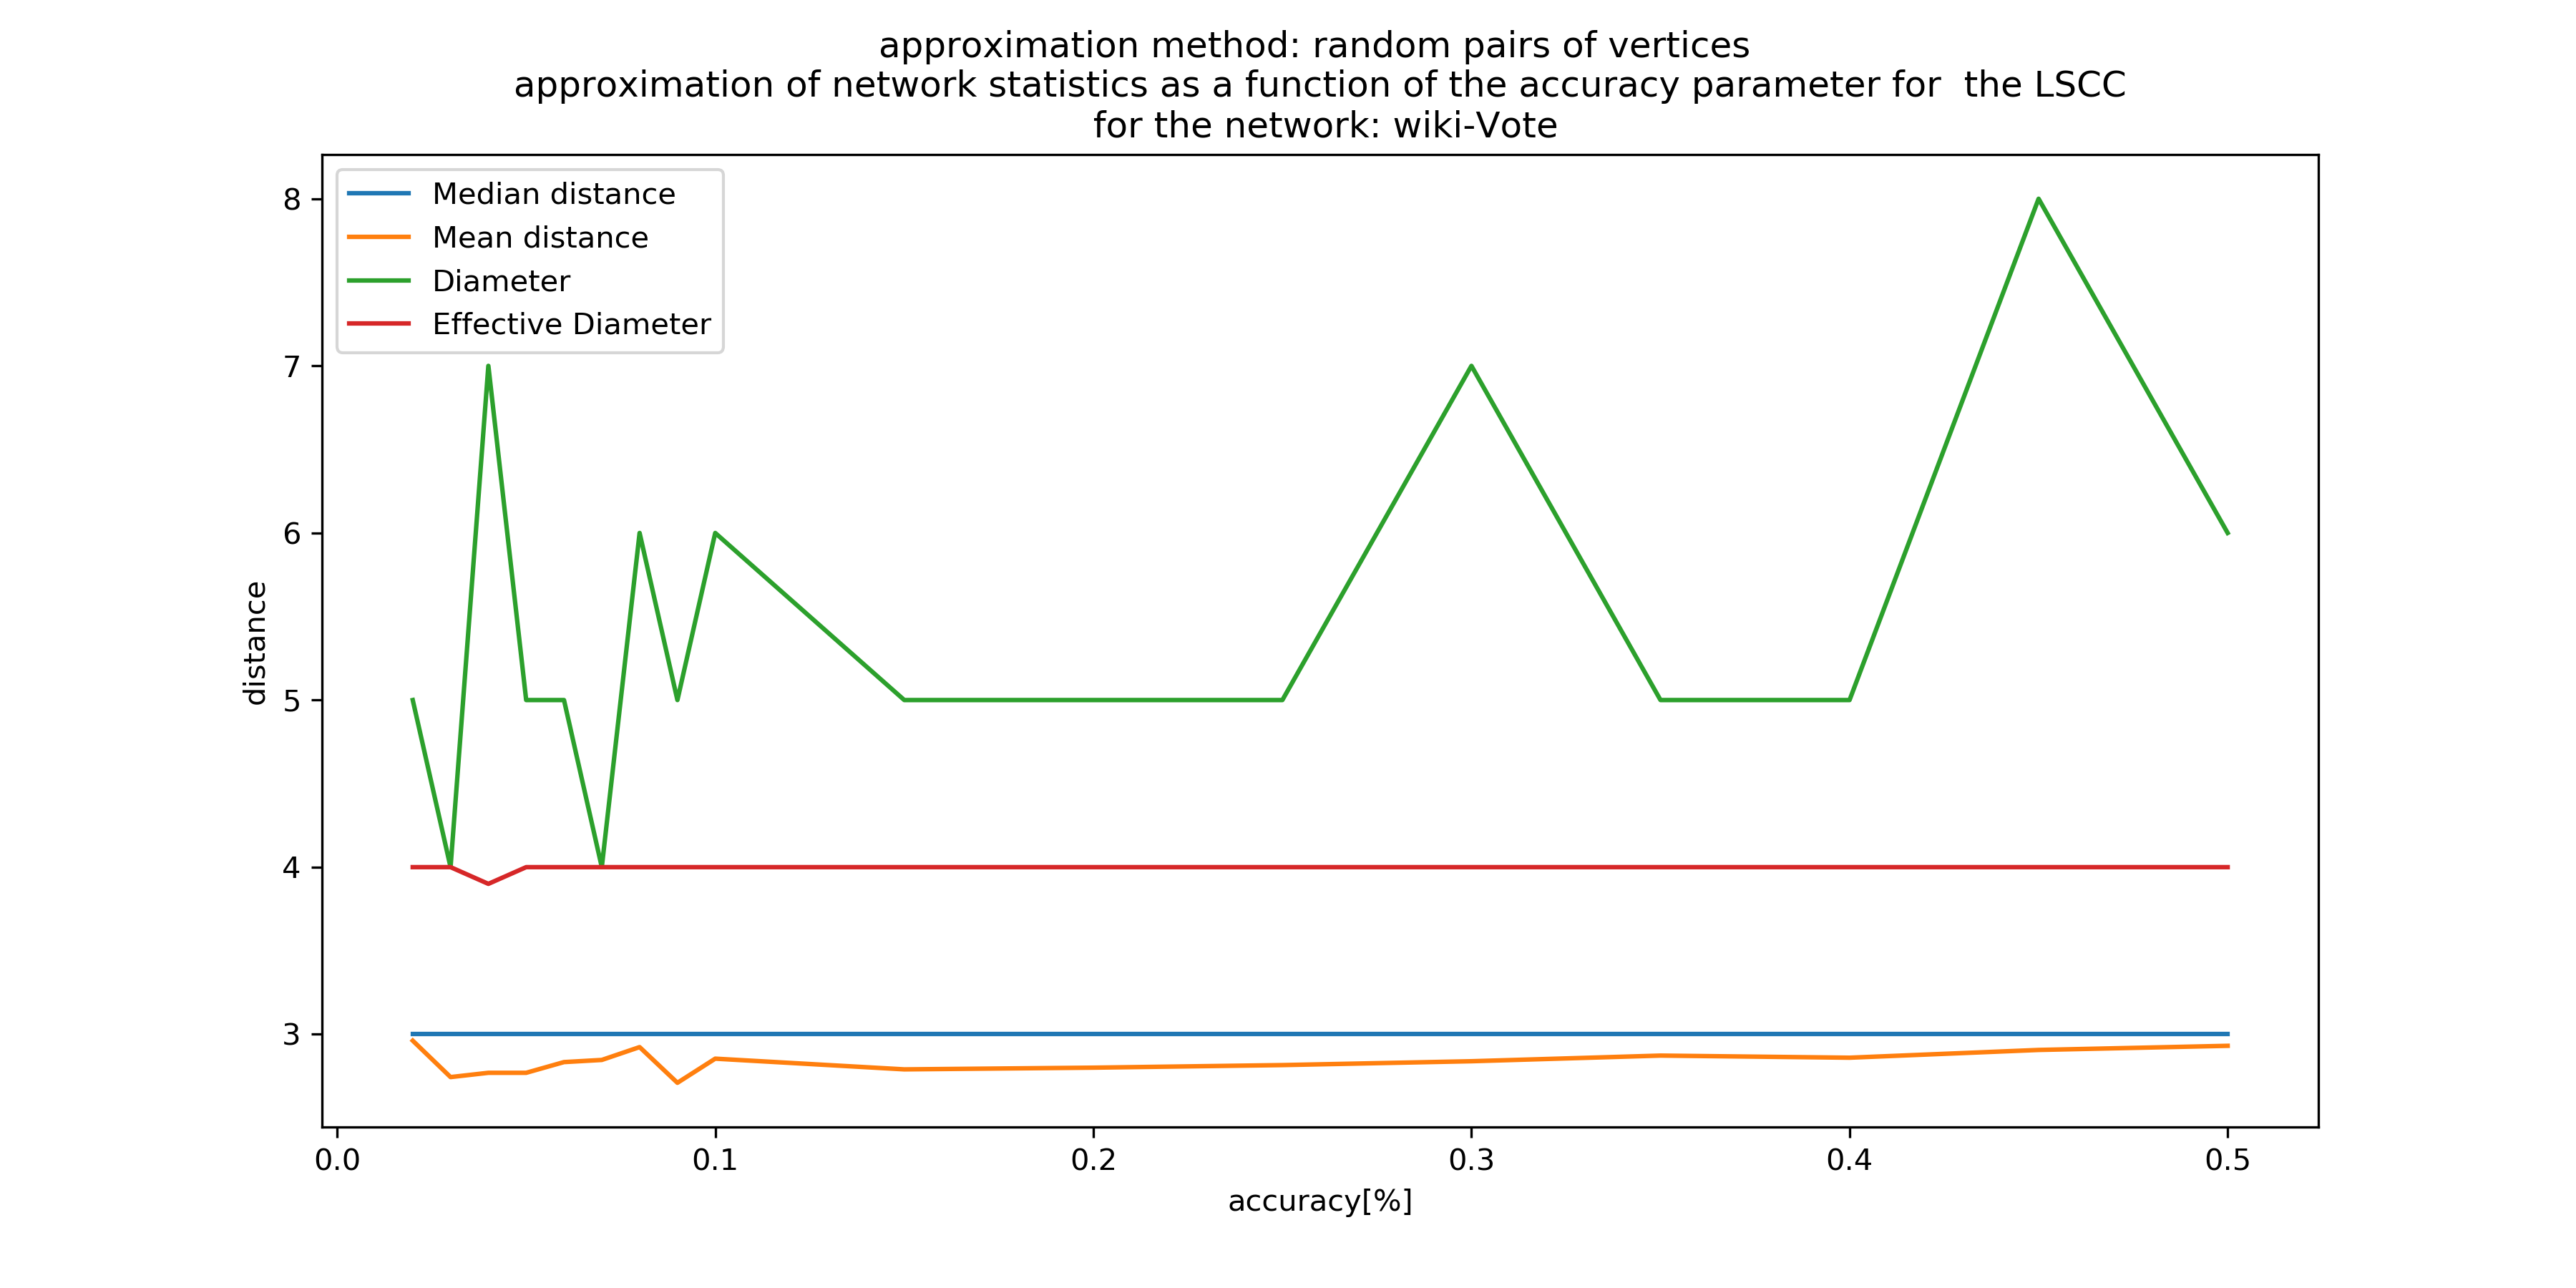
\includegraphics[width=0.9\linewidth]{figures/2_2_wiki-Vote_lscc.png}
\caption{First approximation of the network statistics by \textbf{sampling random pairs of vertices} to approximate network statistics as a function of the accuracy parameter for the \textbf{LSCC} for the network \textit{wiki-Vote}. The dashed line corresponds to the exact value of the network statistics in the same colour.}
\label{pic:2_2_wiki-Vote_lscc}
\end{figure}

\begin{figure}[h!]
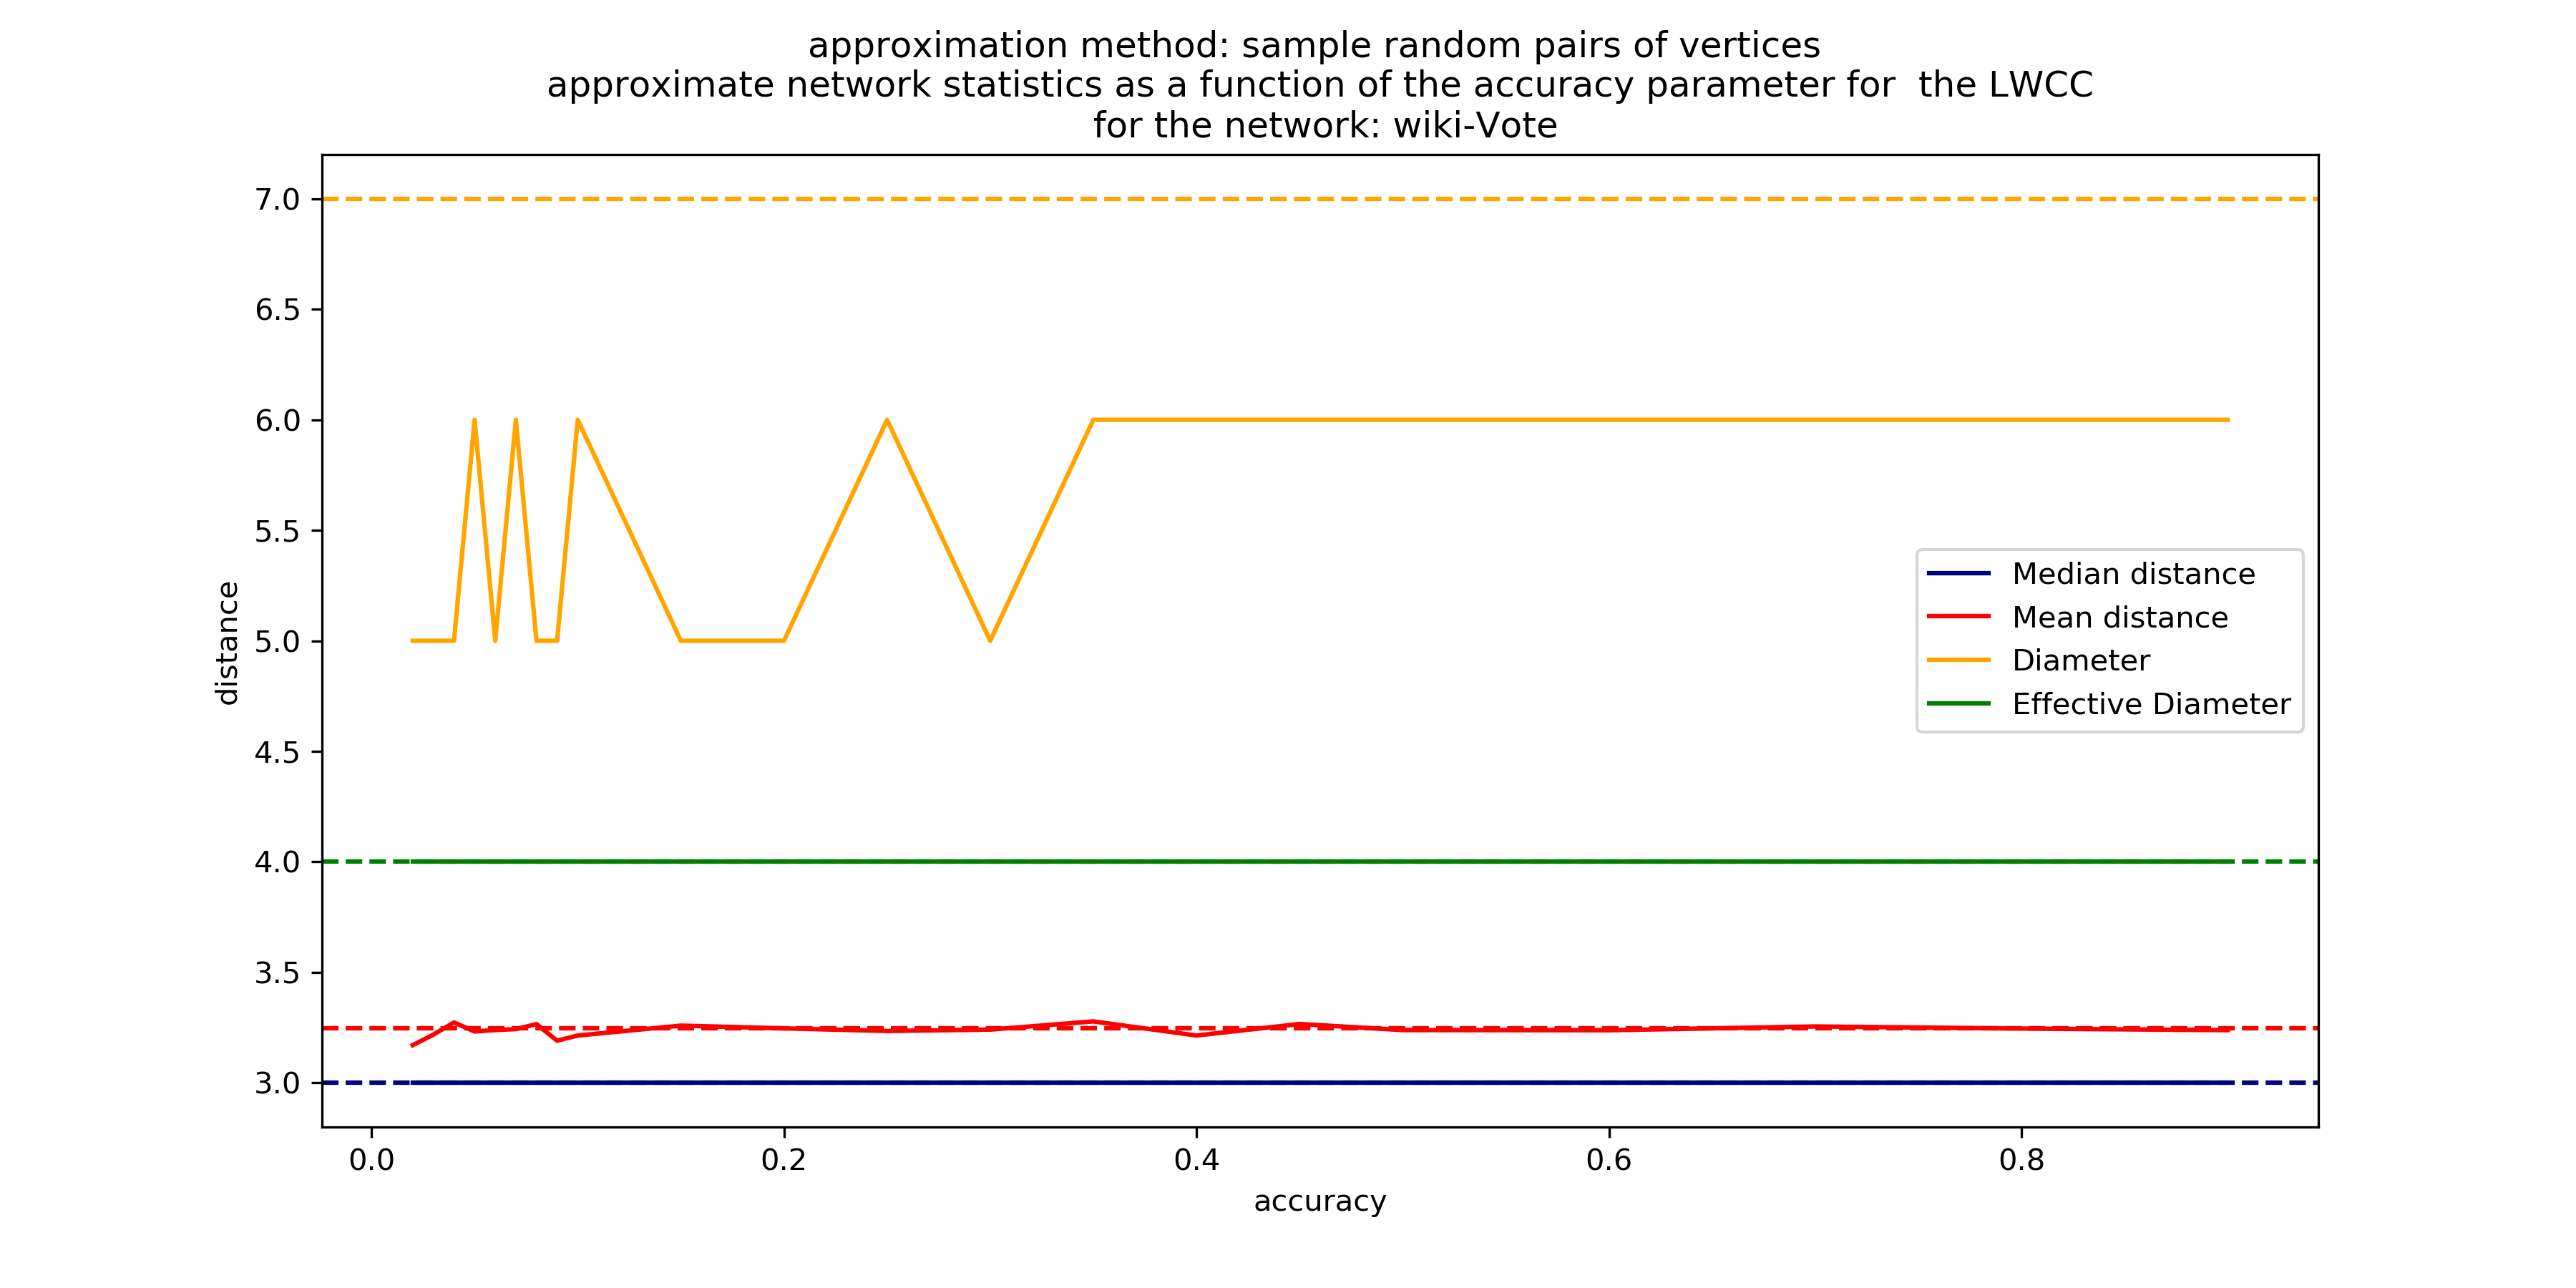
\includegraphics[width=0.9\linewidth]{figures/2_2_wiki-Vote_lwcc.png}
\caption{First approximation of the network statistics by \textbf{sampling random pairs of vertices} to approximate network statistics as a function of the accuracy parameter for the \textbf{LWCC} for the network \textit{wiki-Vote}.The dashed line corresponds to the exact value of the network statistics in the same colour.}
\label{pic:2_2_wiki-Vote_lwcc}
\end{figure}

The Figures~\ref{pic:2_2_wiki-Vote_lscc} and \ref{pic:2_2_wiki-Vote_lwcc} show, that for sampling random pairs of vertices all approximate network statistics apart from the diameter converge already for very small accuracies to the exact value. Therefore a relatively small fraction of the number of vertices can be selected as the number of random sampled pairs and quite accurate approximations for all network statistics but the diameter can be achieved.

\begin{figure}[h!]
	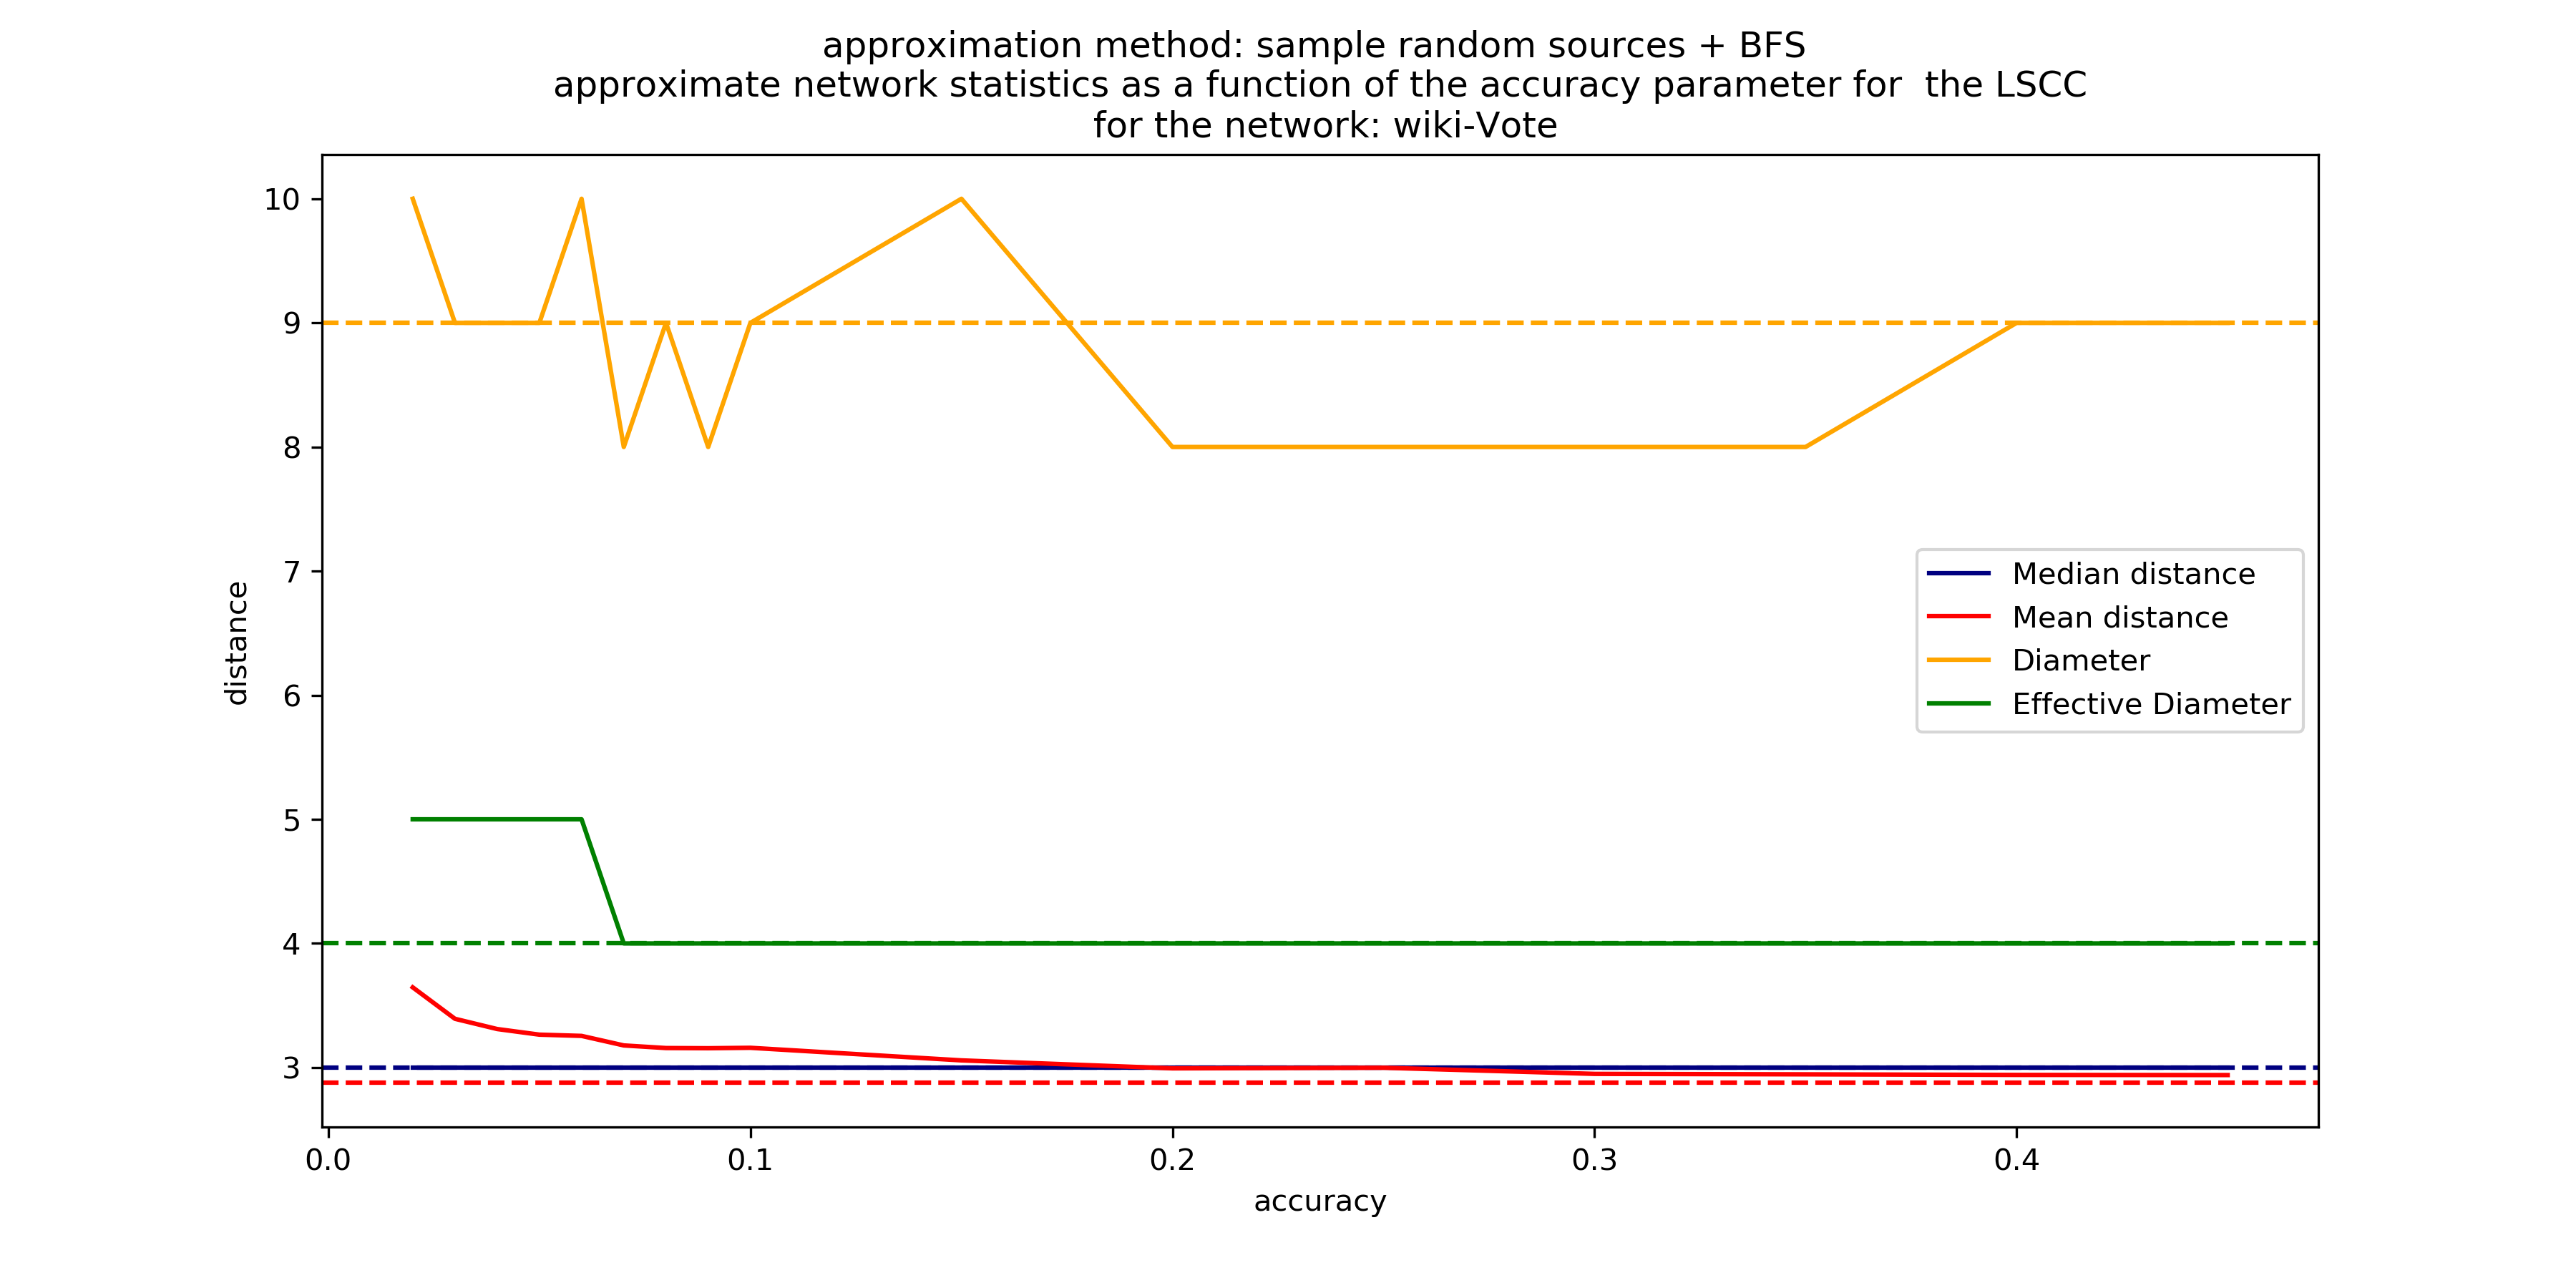
\includegraphics[width=0.9\linewidth]{figures/2_2_method2_wiki-Vote_lscc.png}
	\caption{Second approximation of the network statistics by \textbf{sampling random sources and applying breadth-first search} to approximate network statistics as a function of the accuracy parameter for the \textbf{LSCC} for the network \textit{wiki-Vote}. The dashed line corresponds to the exact value of the network statistics in the same colour.}
	\label{pic:2_2_method2_wiki-Vote_lscc}
\end{figure}

\begin{figure}[h!]
	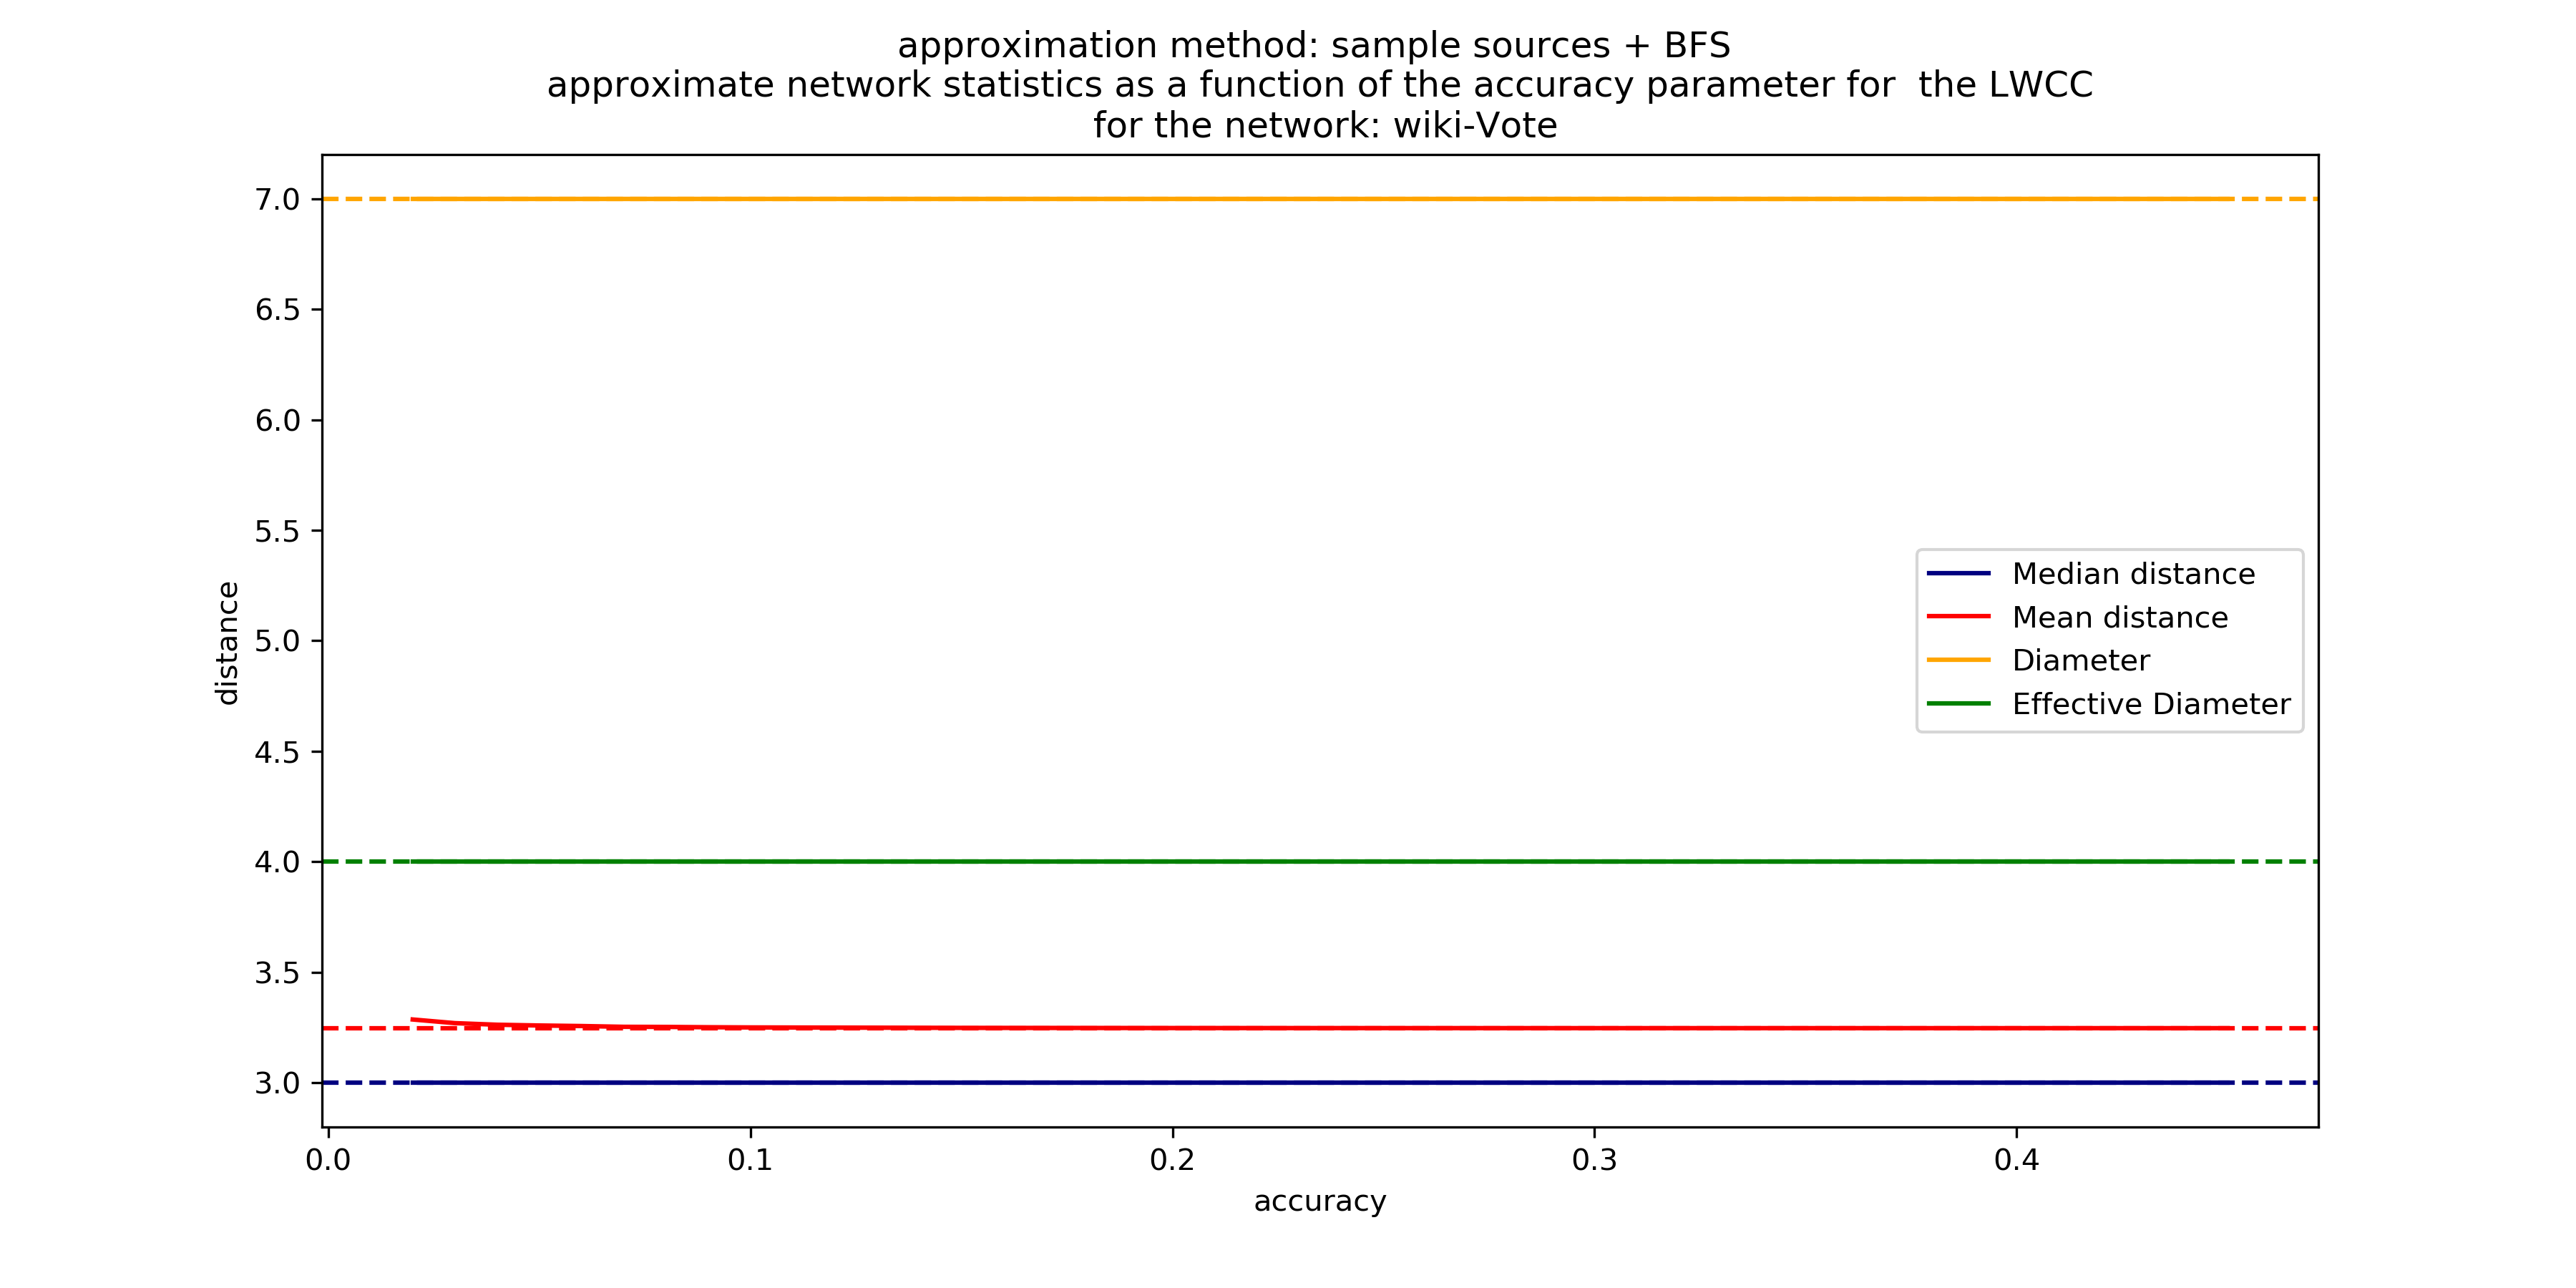
\includegraphics[width=0.9\linewidth]{figures/2_2_method2_wiki-Vote_lwcc.png}
	\caption{Second approximation of the network statistics by \textbf{sampling random sources and applying breadth-first search} to approximate network statistics as a function of the accuracy parameter for the \textbf{LWCC} for the network \textit{wiki-Vote}. The dashed line corresponds to the exact value of the network statistics in the same colour.}
	\label{pic:2_2_method2_wiki-Vote_lwcc}
\end{figure}

\subsection{Discussion}

\begin{enumerate}[(i)]
\item How good is the approximation?

Both approximation methods are surprisingly good. Both achieve good estimations of the exact network statistics already with a small accuracy parameter.

Before having implemented those approximation methods we thought that an accuracy of above 50\% would yield to promising results. But already really small accuracies (less than 5\%) achieve highly accurate estimations of the network statistics. 

The hardest network statistic to estimate is the diameter. This also makes sense as it is a number which represents an important part of the entire graph. Random sampling of pairs of vertices and or BFS might not capture this property. 

\item Which of the three approximation methods is better and why?

The second approximation method looks superior.
For one reason because it takes less accuracy to get to closer values of ground truth than the first approximation method.
And secondly especially early estimations of the diameter are considerably closer to the exact value than the estimation obtained by simple random sampling of pairs of vertices. The approximations method of random sampling of pairs of vertices would need a very high accuracy to predict the diameter with a high confidence, which will be costly in terms of computation. The approximations method of picking random sources and applying breadth-first search on the other hand is predicting accurate estimations starting with low accuracy parameters. 

\item What is the recommended value of the accuracy parameter, according to your experiments?

Judging by the plots displayed in Figure~\ref{pic:2_2_method2_wiki-Vote_lscc} and \ref{pic:2_2_method2_wiki-Vote_lwcc} an accuracy parameter between $0.1$ and $0.2$ seems like a reasonable trade-off between computation time and achieved accuracy of the estimated network statistics.

\end{enumerate}

\end{document}
